\section{Introduction}

\textbf{\color{red}Submission rules}
\begin{itemize}
\color{red}
\item Submission must be in \textbf{PDF format} only.
\item Use a \textbf{two-column format}.
\item The font size for the main text should be \textbf{11}, while the abstract and references can use font size \textbf{9}.
\item Submission is limited to a \textbf{maximum of 4 pages}, including all content (\textbf{strict limit}).
\item Additionally, prepare a \textbf{short abstract} (maximum 150 words) for entry into the online submission system. This abstract will be used for the program only and will not be part of the review process nor the final proceedings.
\end{itemize}

\lipsum[2]

\section{Materials and Methods}
\subsection{Citations}
This is how you add one \cite{Liu2018} or multiple citations \cite{Baete2004,Vunckx2012,Burgos2014}.
\subsection{Equations}
% example equation
And this is a dummy equation \ref{eq:1}.
\begin{equation}\label{eq:1}
I_\alpha = \int_0^\alpha f(x) dx
\end{equation}
\subsection{Figures}
% example two column figure (use figure instead of figure* for one column figure)
\begin{figure*}
  \centering
  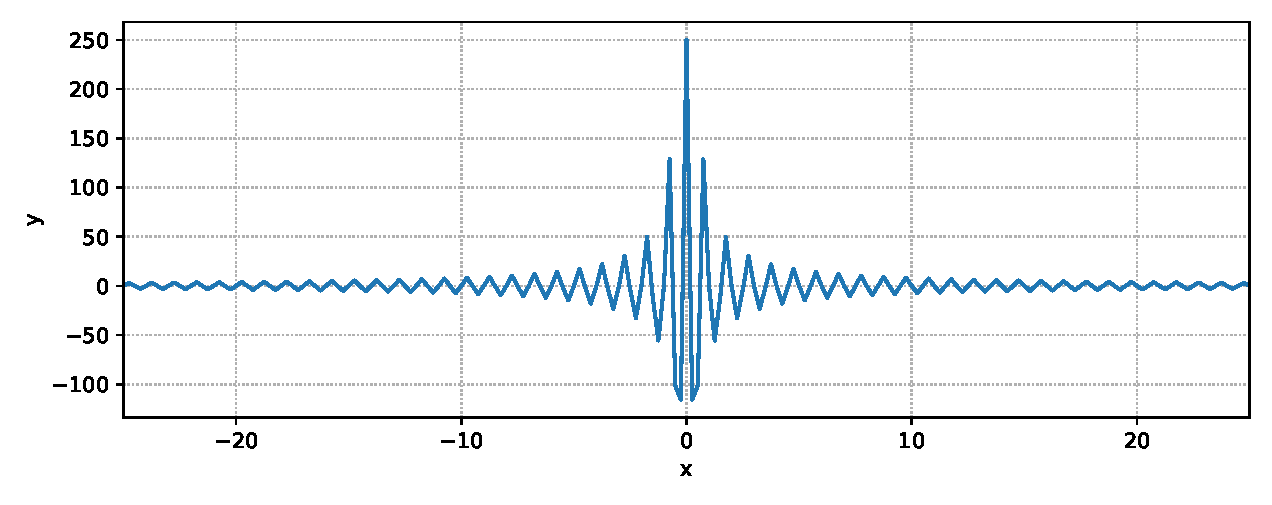
\includegraphics[width=1.0\textwidth]{./fig1.pdf}
  \caption{This a dummy figure to be replaced.}
  \label{fig:dummyfigure}
\end{figure*}

Figure \ref{fig:dummyfigure} shows how to include a figure.
Table \ref{tab:dummytable} shows how to include a table.

\bigskip

\lipsum[2-3]

\section{Results}
\subsection{Simulation results}

\lipsum[2]

\subsection{Other results}
\lipsum[2]

% example table
\begin{table}
  \centering
  \begin{tabular}{lrrr}
  \toprule
  $\alpha$   & $\beta$ & $\gamma$ & $\delta$ \\
  \midrule
  A          & 1       & a        & 3        \\
  B          & 2       & b        & 2        \\
  C          & 3       & c        & 1        \\
  \bottomrule
  \end{tabular}
  \caption{This is a dummy table to be replaced.}
  \label{tab:dummytable}
\end{table}



\section{Discussion}
\lipsum[2]


\section{Conclusion}
\lipsum[2]


